\section{Wakefields}

Wakefields is the conventional name given to the phenomenon of induced electromagnetic fields due to charged particles traversing the beam pipe, RF cavities and many other pieces of equipment facing a particle beam in a particle accelerator. They have long been studied as a source of collective instabilities within particle accelerators \cite{Laslett:ResWallInstab}, through the use of analytical models for different beam pipe geometries \cite{Stupakov:wakeandImp, Stupakov:surfaceRough, Stupakov:adInImpTheory} and materials \cite{Mounet:PhDThesis}, using computational simulation tools, and both beam-based and bench-top measurement techniques. In this chapter is presented a number of significant properties of wakefields and their frequency domain counterpart, beam coupling impedance, as well as a select example of observable effects that wakefields produce.

To aid in the explanation there will first be a short definition of the relative positions and labels of particles used in the following section (this derivation follows the examples given by Stupakov \cite{Stupakov:wakeandImp} and Palumbo \cite{Palumbo:Wakes}). We define the source, or inducing particle as a charged particle with charge $q_{1}$ moving with velocity $\mathbf{v} = \beta{}c \mathbf{\hat{z}}$ at coordinate $\left( \mathbf{r_{1}} \right)$, leading a test, or witness particle, with charge $q_{2}$, moving with velocity $\mathbf{v}$ at coordinate $\left( \mathbf{r_{2}} \right)$ at a distance $z_{1} - z_{2}$ behind the source particle. This relationship is visualised in Fig.~\ref{fig:source_and_wit}.

\begin{figure}
\begin{center}
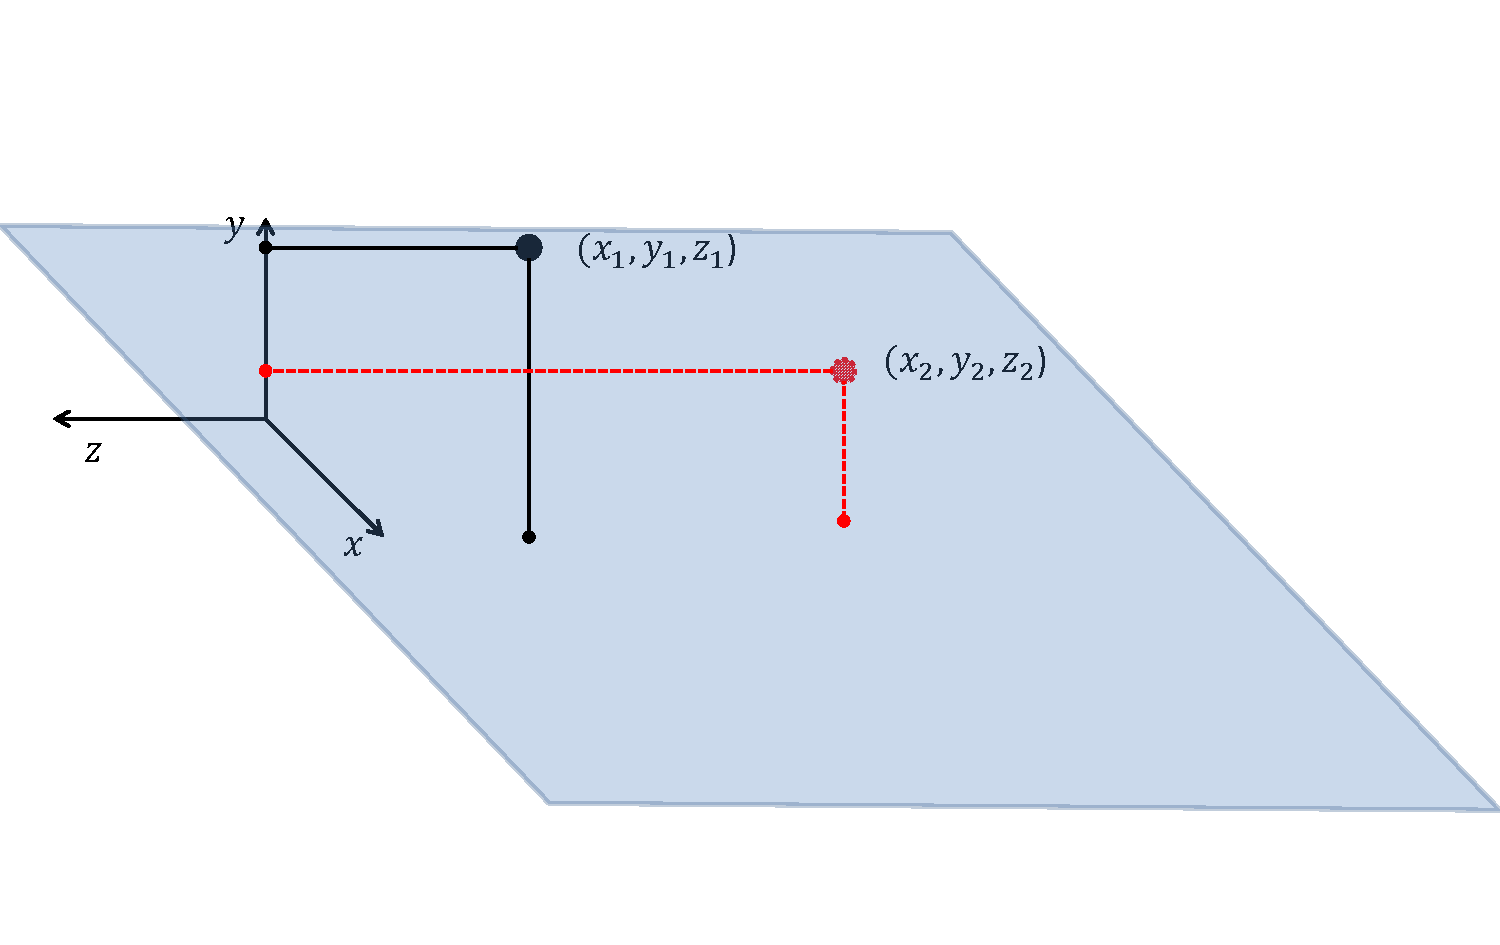
\includegraphics[width=0.85\textwidth]{Wakefields_and_Impedances/figures/source-witness-pos.pdf}
\end{center}
\caption{The relative displacements and velocities of the source (S) and test (T) particles.}
\label{fig:source_and_wit}
\end{figure} 

\subsection{The Electromagnetic Fields of a Moving Charged Particle in Free Space}

If we consider the electromagnetic fields generated by the source particle, it can be shown that the fields at a vector $\mathbf{R} = \mathbf{r_{1}} - \mathbf{r_{2}}$ are given by

\begin{align}
\mathbf{E}\left( \mathbf{R}  \right) = \frac{q_{1}\mathbf{R}}{\gamma^{2}\left| \mathbf{R} \right|^{3}} \\
\mathbf{H}\left( \mathbf{R}  \right) = \frac{1}{c}\mathbf{v} \times \mathbf{E}
\label{eqn:gen_fields_mov_part}
\end{align}

where $\gamma =(1- v^{2}/c^{2})^{-1/2}$ is the relativistic gamma factor. It can be shown that, if we take the ultrarelativistic limit (i.e. $\gamma \rightarrow \infty$) we can see that Eqn~\ref{eqn:gen_fields_mov_part} becomes

\begin{equation}
\mathbf{E}\left( \mathbf{R}  \right) = \frac{2q_{1}\mathbf{r}}{r^{3}}\delta{z-ct} \\
\mathbf{H}\left( \mathbf{R}  \right) = \mathbf{\hat{z}} \times \mathbf{E}
\label{eqn:ultrarel_field_eqn}
\end{equation}

where $\mathbf{r} = x\mathbf{\hat{x}} + y\mathbf{\hat{y}}$ is a purely transverse vector.

The following witness particle experiences the resulting Lorentz force 

\begin{equation}
\mathbf{F}\left(\mathbf{r_{1}}, \mathbf{r_{2}}  \right) = q_{2}\left[ \mathbf{E} + \mathbf{v} \times \mathbf{B}  \right]. 
\end{equation}

Looking at Eqn.~\ref{eqn:ultrarel_field_eqn}, it can be seen that the force can be seperated into longitudinal and transverse components 

\begin{align}
F_{\parallel}\left(\mathbf{r_{1}}, \mathbf{r_{2}}  \right) = q_{2}E_{\parallel} \\
\mathbf{F_{\perp}}\left(\mathbf{r_{1}}, \mathbf{r_{2}}  \right)  = q_{2}\left[ \mathbf{E_{\perp}} + \left( \mathbf{v} \times \mathbf{B} \right) \right]
\end{align}

where $\mathbf{E_{\perp}} = E_{x}\mathbf{\hat{x}} + E_{y}\mathbf{\hat{y}}$. $F_{\parallel}$ has only an electric component as the magnetic flux density $\mathbf{B}$ has magnitude = 0 in the $\mathbf{\hat{z}}$ direction. Considering just the longitudinal force, integrating over all space gives the total energy change of the source particle

\begin{equation}
U_{1}\left(\mathbf{r_{1}}  \right) = - \int^{\infty}_{-\infty} d\mathbf{z} . \mathbf{F}\left(\mathbf{r_{1}}  \right)
\end{equation}

where $F( \mathbf{r_{1}} ) = q_{1} E (\mathbf{r_{1}} )$. Similarly the energy change in the witness particle can be calculated by

\begin{equation}
U_{2}\left(\mathbf{r_{1}}, \mathbf{r_{2}}, \tau  \right)  = - \int^{\infty}_{-\infty} d\mathbf{z} \mathbf{F}\left(\mathbf{r_{1}}, \mathbf{r_{2}}  \right)
\label{eqn:witness_energy_change_single}
\end{equation}

where $\tau = \left( z_{1}-z_{2} \right)/(\beta{}c)$ and $F( \mathbf{r_{1}}, \mathbf{r_{2}} ) = q_{2} E (\mathbf{r_{1}}, \mathbf{r_{2}} )$. From these two energy losses two widely used terms can be extracted; the loss factor $k$, given by

\begin{equation}
k_{loss}\left(\mathbf{r_{1}}  \right) = \frac{U_{1}\left(\mathbf{r_{1}}  \right)}{q_{1}^{2}}
\end{equation}

and the longitudinal wake function, given by

\begin{equation}
w_{\parallel}\left(\mathbf{r_{1}}, \mathbf{r_{2}}, \tau   \right) = \frac{U_{2}\left(\mathbf{r_{1}}, \mathbf{r_{2}}, \tau  \right) }{q_{1} q_{2}},
\label{eqn:long_wake_func}
\end{equation}

denoting the normalised (with respect to source charge, and source and witness charge respectively) energy change of both the source particle (loss factor) and witness particle (wake function). 

\subsection{Wakefields of a Bunch}

As colliders are often used to collide bunches of particles as opposed to single particles, it is useful to be able to define the wake function of a bunch distribution. It can be seen that the total source charge of a bunch $q_{1}$ is the integral of the longitudinal current distribution $i_{b}\left( \tau \right)$ integrated over all time

\begin{equation}
q_{1} = \int^{\infty}_{-\infty}i_{b}\left( \tau \right) d\tau{}.
\end{equation}

The wake function of a bunch distribution at a point at time $\tau$ can be calculated by the convolution of the single particle wake function with the bunch distribution. Thus, if the bunch is split into infinitesimally small slices, the change in energy of a witness particle of charge $q$ at time $\tau$ due to a slice at time $\tau{}'$ is given by

\begin{equation}
dU\left(\mathbf{r_{2}}, \tau-\tau{}'  \right) = q i_{b}\left( \tau{}' \right) w_{\parallel}\left( r_{2}, \tau{}-\tau{}' \right).
\end{equation}

The longitudinal bunch wake function $W_{\parallel}\left(\mathbf{r_{2}}\right)$ can then be calculated using Eqn.~\ref{eqn:witness_energy_change_single}

\begin{equation}
W_{\parallel}\left( \mathbf{r_{2}}, \tau \right) = \frac{U\left( r_{2}, \tau \right) }{q_{1} q_{2}} = \frac{1}{q_{1}}\int^{\infty}_{-\infty}i_{b}\left( \tau{}' \right) w_{\parallel}\left( r_{2}, \tau{}-\tau{}'\right) d\tau{}' .
\end{equation}

\subsection{Transverse Wakefields}

Similar to the longitudinal wakefield, we can see that the total tranverse momentum change of the witness particle is given by integrating the transverse force across all space

\begin{equation}
\mathbf{P}\left(\mathbf{r_{1}}, \mathbf{r_{2}}, \tau  \right) = \int^{\infty}_{-\infty} \mathbf{F_{\perp}} \left( \mathbf{r_{1}},  \mathbf{r_{2}}\right) dz
\end{equation}

where $\tau$ is the time delay between source and witness particles. And similarly to the longitudinal plane we can define a wake function normalised with regards to the source and witness particle charges

\begin{equation}
\mathbf{w_{\perp}}\left(\mathbf{r_{1}}, \mathbf{r_{2}}, \tau  \right) = \frac{\mathbf{P}\left(\mathbf{r_{1}}, \mathbf{r_{2}}, \tau  \right)}{q_{1} q_{2}}.
\label{eqn:trans_wake_func}
\end{equation}

And in a similar manner to the longitudinal bunch wake function a form for the transverse bunch wake function can be derived

\begin{equation}
W_{\perp}\left( \mathbf{r_{2}}, \tau \right) = \frac{U\left( r_{2}, \tau \right) }{q_{1} q_{2}} = \frac{1}{q_{1}}\int^{\infty}_{-\infty}i_{b}\left( \tau{}' \right) w_{\perp}\left( r_{2}, \tau{}-\tau{}'\right) d\tau{}' .
\end{equation}

\subsection{Panowsky-Wenzel Theorem}
\label{sec:PanWen}

Considering the force acting on the witness particle by the Lorentz force, it can be seen that the force is given by 

\begin{equation}
\mathbf{F} = q_{2} \left[\mathbf{E} + \mathbf{v}\times \mathbf{B} \right].
\label{eqn:wit_gen_force}
\end{equation}

Now, considering Faraday's law in integral form ($\mathbf{B} = -\int^{t_{2}}_{t_{1}} \left( \nabla \times \mathbf{E} \right) dt$, $t_{1}$ being sufficiently in the past that $\nabla \times \mathbf{E} \rightarrow 0$), Eqn.~\ref{eqn:wit_gen_force} can be rewritten as

\begin{equation}
\mathbf{F} = q_{2}  \left[\mathbf{E} - \mathbf{v}\times\left(  \int^{t_{2}}_{t_{1}} \nabla \times \mathbf{E} dt \right) \right].
\end{equation}

Now, using the fact that the velocity $\mathbf{v}$ is constant and Lagrange's formula (shown in Eqn.~\ref{eqn:lagrangeEqn}) this then becomes

\begin{equation}
\mathbf{F} = q_{2}  \left[\mathbf{E} - \int^{t_{2}}_{t_{1}}\left(  \nabla \left( \mathbf{v} . \mathbf{E} \right)  - \mathbf{v}\left( \nabla . \mathbf{E} \right) \right) dt  \right].
\end{equation}

\begin{equation}
\mathbf{a} \times \left( \mathbf{b} \times \mathbf{c} \right) = \mathbf{b} \left( \mathbf{a}.\mathbf{c} \right) - \mathbf{c}\left( \mathbf{a}.\mathbf{b} \right)
\label{eqn:lagrangeEqn}
\end{equation}

If this force is seperated into the longitudinal and transverse components we see that they are the following

\begin{align}
F_{\parallel} = q_{2} E_{z} \\
\mathbf{F}_{\perp} = q_{2}  \left[\mathbf{E_{\perp}} - v \int^{t_{2}}_{t_{1}}\left(  \nabla_{\perp}E_{z}  - \frac{\partial\mathbf{E}_{\perp}}{\partial z} \right) dt  \right]
\end{align}

where $\nabla_{\perp}$ in the differential operator only in the transverse coordinates. If these are now compared to the identities of the wake function for the longitudinal and transverse wake functions given in Eqns.~\ref{eqn:long_wake_func} and \ref{eqn:trans_wake_func} respectively, it can be seen that

\begin{align}
w_{\parallel}\left( \mathbf{r_{1}}, \mathbf{r_{2}}, \tau   \right) = -\frac{1}{q_{1}} \int^{\infty}_{-\infty} dz E_{z} \left( \mathbf{r_{1}}, \mathbf{r_{2}} \right) \\
\mathbf{w}_{\perp} \left(\mathbf{r_{1}}, \mathbf{r_{2}}, \tau   \right) = \frac{1}{q_{1}} \int^{\infty}_{-\infty} dz \left[ \mathbf{E_{\perp}}\left(\mathbf{r_{1}}, \mathbf{r_{2}} \right) - v   \int^{t_{2}}_{t_{1}}\left(  \nabla_{\perp}E_{z}\left(\mathbf{r_{1}}, \mathbf{r_{2}} \right)  - \frac{\partial\mathbf{E}_{\perp}\left(\mathbf{r_{1}}, \mathbf{r_{2}} \right)}{\partial z} \right) dt \right] \label{eqn:trans_wake_middle}.
\end{align}

The next stage requires partially differentiating Eqn~\ref{eqn:trans_wake_middle} by $s = v \tau = vt - z$. It can be seen from this relationship that $\partial / \partial s = - \partial / \partial z$ and $\partial / \partial s = 1/v \partial / \partial z$. Thus the first term can be replaced by $\partial / \partial s = - \partial / \partial z$, and the term in the interior integral becomes the value of the intergrand at $\tau$.

\begin{equation}
\frac{\partial}{\partial s}\mathbf{w}_{\perp} \left(\mathbf{r_{1}}, \mathbf{r_{2}}, \tau   \right) = \frac{1}{q_{1}} \int^{\infty}_{-\infty} dz \left[ \frac{-\partial}{\partial z}\mathbf{E_{\perp}} + \left(  \nabla_{\perp}E_{z} + \frac{\partial\mathbf{E}_{\perp}}{\partial z} \right) \right].
\end{equation} 

It can be seen that the first and third integrand cancel. Also, the operator $\nabla_{\perp}$ may be moved to the front of the operation without changing the equation, thus

\begin{equation}
\frac{\partial}{\partial s}\mathbf{w}_{\perp} \left(\mathbf{r_{1}}, \mathbf{r_{2}}, \tau   \right) =  \frac{1}{q_{1}} \int^{\infty}_{-\infty} dz \nabla_{\perp}E_{z} = \mathbf{\nabla_{\perp}} w_{\parallel}\left( \mathbf{r_{1}}, \mathbf{r_{2}}, \tau   \right).
\end{equation}

%\begin{itemize}
%\item{Introduction to the electromagnetic field of charged particle moving in free space}
%\item{Field of a particle in a perfectly conducting pipe - method of image currents}
%\item{Place a witness particle distance s behind source particle and deduce electric field as seen by this particle}
%\item{normalise this by the source particle charge to give the wakepotential}
%\item{And again by the source particle charge and current profile to acquire the loss factor}
%\item{Longitudinal field predominantly}
%\item{Introduce the Panowsky-Wenzel theorem covering transverse field - Transverse wakes}
%\end{itemize}
